\chapter{Temporal network analysis}\label{sec:temporal_networks}
The previous chapter has demonstrated that network analysis provides a deep insight into the processes behind epidemic spreading.
Given a sufficient amount of data, a contact network is capable to capture all possible infection pathways in the system.
The potential of static network analysis lies in the huge toolbox of methods that has been developed in the last decades.
As depicted in section \ref{sec:network_theory}, there exist coherent definitions for both their large scale topological features and local centrality measures allowing for node rankings.

Nevertheless, the concept of static networks neglects temporal variations in the system, i.e. the edges of a particular network are not necessarily present all the time.
This chapter addresses some of the conceptional problems owing to a sparse and heterogenous occurrence of edges in the network, the most central one being the \emph{causality of paths} in the network.
Section \ref{sec:Plos} focusses on the computational analysis of the full temporal representation of the network analyzed (from the static perspective) in section \ref{sec:network_analysis}.
In section \ref{sec:PRL}, we present a novel formalism mapping the causality of temporal networks onto a mathematical graph.

\section{Introduction}
To begin with, we highlight the most fundamental difference between static and temporal networks.
In particular, we compare the static and the temporal representation of the system.
Figure \ref{fig:temporal_network_principle} shows a temporal network and its aggregated graph.
%
\begin{figure}[htb]
\begin{center}
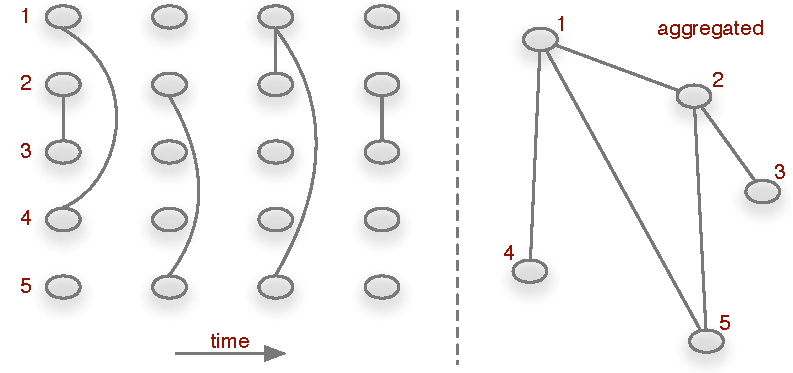
\includegraphics{Temporal_Network_Principle.pdf}
\caption{%
Role of causality in a temporal network with $5$ nodes and $4$ snapshots.
The left panel shows snapshots of the system at different times and the right panel shows the corresponding aggregated network.
Although there is a path from node $3$ to $4$ (and vice versa) in the aggregated network (right panel), there is no causal path between $3$ and $4$ in the temporal network (left panel).
}
\label{fig:temporal_network_principle}
\end{center}
\end{figure}
%
Although the edges of the temporal network are present in the aggregated graph, the situation becomes more complex, if we consider paths of length greater than one.
The aggregated graph (right panel in figure \ref{fig:temporal_network_principle}) suggests that the network is connected, i.e. there is a path between every node pair.
As an example, there are two different paths from node $3$ to $4$ in the aggregated system.
However, this does not hold for the temporal system.
Consequently, paths in an aggregated graph of a temporal network have to be treated with care.

Before we give a formal definition of temporal networks, we have to distinguish between terms used for temporal networks and other systems.

\paragraph{Disambiguation\color{Cayenne}{.}}
Since the analysis of temporal networks is an interdisciplinary field, there is still no consistent designation for what the author refers to as \emph{temporal networks} \citep{Holme_review}.
Different phrases, such as temporal graphs, dynamic graphs, dynamic networks are used in the literature.
In addition to that, there are other classes of networks seeming to be related to temporal networks, i.e. adaptive networks, growing networks, evolving graphs.
The analysis of the latter has a strong focus on network growth, i.e. the process behind the evolution of static networks.
A central question for these systems is what is the fundamental process that has formed the network.
An example is the \BA network, where the underlying process is a rich-get-richer principle that results in a scale free degree distribution.
The striking difference between growing networks and temporal networks is that the snapshots of a temporal network can in principle be arbitrary.
Correlations between two snapshots of the system (if any) could be over arbitrary periods of time.
We prefer the term temporal network, since \emph{temporal} is not so easily confused with dynamic systems.
Furthermore, the systems under consideration are not mathematical graphs; therefore, we use the more general term \emph{network}.

\subsection{Formal definition}
A temporal network $\mathcal{G}=(V,\mathcal{E},T)$ consists of a set of nodes $V$ and a set of edges $\mathcal{E}$, where each edge in $\mathcal{E}$ is given by a triple $(u,v,t)$ and connects nodes $u$ and $v$ at time $t\in T$.
$T$ is the observation period of $\mathcal{G}$, where $T\subset \mathbb{N}^+$ for time discrete systems and $T\subset \mathbb{R}^+$ for continuous systems.
\footnote{
In this work, we focus on time discrete systems, since a continuous time process can be approximated by a discrete one by choosing an appropriately small increment.
Furthermore, edge weights and a latency functions for edge traversal could be added to the definition \citep{Casteights_review}.
This is, however, beyond the scope of this thesis.
}
The aggregated graph $G=(V,E)$ of a temporal network simply ignores the occurrence times of the edges in $\mathcal{E}$ and the set of nodes $V$ is the same in both representations.
%
In analogy to static networks, we denote the \emph{transitive closure} of $\mathcal{G}=(V,\mathcal{E},T)$ by $\mathcal{G}^*=(V,\mathcal{E}^*,T)$, where $\mathcal{E}^*$ contains an edge $(u,v,t)$, wherever there is a causal path from node $u$ to $v$ arriving at time $t$ and having started at some time $t_0<t$.
%
Following \citep{Casteights_review}, the \emph{horizon} $\mathcal{H}$ of node $u$ is defined by the set
\begin{equation}\label{eq:temporal_horizon}
\mathcal{H}_u = \left\{ v: \exists \; u\rightsquigarrow v  \right\},
\end{equation}
where $ u\rightsquigarrow v $ means that there is a causal path from node $u$ to $v$.

\subsection{Viewpoints and implementation}
As in the case of static networks, temporal networks can be interpreted and implemented in different ways \citep{Casteights_review}.
A brief report of different implementations of static networks is given in Appendix \ref{sec:implementation}.
Besides the adjacency matrix, edge lists and adjacency lists are appropriate network representations.
Considering a temporal network as a sequence of static networks (called snapshots or graphlets) can be seen as a \emph{graph centric} view on the system.
It is the analogue of the adjacency matrix in static networks.
More formally, a temporal network $\mathcal{G}$ is represented by a sequence of adjacency matrices
\begin{equation}\label{eq:AdMatrixSequence}
\mathcal{A}=\mat{A}_1,\dots ,\mat{A}_T,
\end{equation}
where $T$ is the observation time and the increment is the temporal resolution.

In analogy to the edge lists of static networks (see Appendix \ref{sec:implementation}), an \emph{edge centric} view on a temporal network consists of the occurrence times of the edges.
Let $\mathcal{G}=(V,\mathcal{E})$ be a temporal network.
Than the set of edges $\mathcal{E}$ is represented by a sequence of triples
\begin{equation*}%\label{eq:temporal_edges}
\mathcal{E}=(u_1,v_1,t_1),(u_1,v_1,t_2),(u_2,v_2,t_2),\dots \;.
\end{equation*}
An edge centric view focusses on the occurrence times of each edge, i.e.
\[
\mathcal{I}((u_1,v_1))=t_2,t_2,\dots \; .
\]
This point of view is particularly convenient for the time randomization of temporal networks (see section \ref{sec:randomized_models_tvg}).
Finally, a \emph{node centric} view of a temporal network considers the neighborhood $\mathcal{N}$ of a node $v$ over time, i.e. $\mathcal{N}(v,t)$.
This view corresponds to the adjacency list of a static network (see Appendix \ref{sec:implementation}).
The temporal degree of each node immediately follows from $d(v,t)=\abs{\mathcal{N}(v,t)}$.
The edge centric and node centric network view is considered as a microscopic perspective, while the graph centric view provides a macroscopic perspective.

We make use of microscopic perspective implicitly in computer implementations as in section \ref{sec:Plos}.
Furthermore, we focus on the graph centric view \eqref{eq:AdMatrixSequence} in section \ref{sec:PRL} to analyze macroscopic path structures in temporal networks.

\subsection{Paths in temporal networks}\label{sec:paths_in_temporal_networks}
A causal sequence of edges between two nodes $u$ and $v$ in a temporal network is called (causal) path.
It is given by a sequence of edges, i.e.
\[
\mathrm{path}(u,v,t)= \{ (u,x,t_1),(x,y,t_2),\dots ,(z,v,t_n) \}, 
\]
where $ t_1<t_2<\dots <t_n$ and $x$, $y$ and $z$ are nodes on the path.
It is interesting to note that paths in a temporal network are in general \emph{not transitive}.
Transitive means that the existence of a path from node $u$ to $v$ and a path from $v$ to $w$ implies that there is a path from $u$ to $w$, i.e.
\begin{equation}\label{eq:def_transitive}
(u\rightarrow v) \wedge (v\rightarrow w) \; \Longrightarrow \; (u\rightarrow w).
\end{equation}
This property is obviously satisfied for all static networks.
In temporal networks, however, paths are in general not transitive, since a path from $u$ to $v$ could simply exist only at a later time than the path from $v$ to $w$, so that
\begin{equation}\label{eq:def_not_transitive}
(u\rightsquigarrow v) \wedge (v\rightsquigarrow w) \;\centernot \Longrightarrow \; (u\rightsquigarrow w)
\end{equation}
in general.
The reasons why paths in temporal networks can not be easily represented by paths in static networks originate from property \eqref{eq:def_not_transitive}.
In section \ref{sec:conceptual_problems} we briefly discuss some conceptual problems that arise from this circumstance.


\begin{SCfigure}
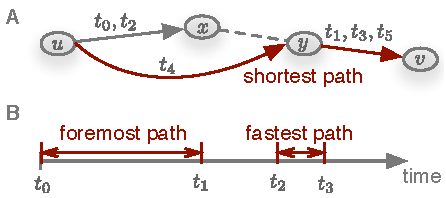
\includegraphics{Shortest_foremost_fastest.pdf}
\caption{Topological shortest distance and temporal shortest durations for a path between nodes $u$ and $v$.
The shortest path (panel A) counts the number of edges between the nodes.
Panel~B demonstrates that although the fastest path could take $t_3-t_2 < t_1-t_0$, the foremost path arrives already at $t_1<t_2$.
}
\label{fig:shortest_foremost_fastest}
\end{SCfigure}
%
Note that possible paths between nodes depend on time in general.
This has crucial implications on the \emph{shortest path distance} known from static networks (see section  \ref{sec:network_terminology}).
As a matter of fact, there are three different shortest path types in temporal networks.
Just like in the static case, the shortest path distance between two nodes measures the topological distance between the nodes.
It counts the number of edges used do traverse the shortest path.
In addition, the \emph{duration} of a path can be measured in temporal networks.
This duration can be measured in two different time frames \citep{Casteights_review}:
First, the \emph{fastest} path between two nodes is the path of shortest duration, no matter when the path starts in time.
Second, the \emph{foremost} path between two nodes is the path that arrives earliest in a global time frame.

Figure \ref{fig:shortest_foremost_fastest} demonstrates the difference between the foremost, fastest and shortest path concept, respectively.
Edge labels are edge occurrence times, which are ordered so that $t_1<t_2<t_3<t_4<t_5$.
The dashed edge $(x,y)$ indicates that these nodes are not connected directly, but by other nodes of the network.
Panel A shows that the shortest topological path between nodes $u$ and $v$ is $(u,x,v)$ and the distance is $3$.
It can be seen from panel B that the first (foremost) path start at node $u$ at time $t_0$ and arrives at node $v$ at time $t_1$.
Although the fastest path takes less time to traverse ($t_3-t_2<t_1-t_0$), it arrives later ($t_3>t_1$) than the foremost path.
Note that shortest path and temporal shortest path do not coincide in this example, since the shortest path connection can be at times $t_4$ and $t_5$ which are greater than $t_1$ and $t_3$.

Throughout the rest of this work, we use a global time scale, which is defined by the first time in the dataset under consideration.
Consequently, we measure shortest path durations in terms of \emph{foremost} path durations, if not explicitly stated.

\subsection{Conceptual problems in temporal networks}\label{sec:conceptual_problems}
Before we focus on different methods to analyze temporal networks, we have to point out that many static network measures, such as centrality or components, are in general time-dependent and can not be summarized to single numbers.
In addition, time-scales of node dynamics and network dynamics can be of the same order and cause significant interactions between the dynamics.
We consider the relation between node dynamics and edge dynamics in section \ref{sec:Plos}.

The most essential difference between static and temporal networks lies in the importance of causality of paths in temporal networks.
Although it is possible to analyze paths in temporal networks systematically (see section \ref{sec:PRL}) we have to stress that generalizing the concept of connected components is far more complex in temporal networks.
\citeauthor{Nicosia:2012hz} point out that finding connected components in temporal networks is NP-complete in general \citep{Nicosia:2012hz}.
In addition to that, the authors demonstrate that components in temporal networks can be \emph{degenerated}, i.e. there are multiple possible partitions of connected components and nodes can belong two multiple components at the same time.

We take up this point at the end of section \ref{sec:PRL}.
In order to get an impression about paths in temporal networks, we start with a pure data-analysis of a temporal network dataset. 



\section{Data driven network analysis}\label{sec:Plos}
In this section we analyze the pig trade data set as introduced in section \ref{sec:network_analysis}, but we explicitly take into account temporal information%
\footnote{%
In order to be congruent with the datasets used in the publications, we use the pig trade dataset of \citep{Konschake:2013js} in this chapter.
This dataset differs slightly from the dataset used in section \ref{sec:network_analysis}.
It covers the period from 01 January 2008 to 31 December 2009.
The results do not change qualitatively and hereby the results of \citep{Konschake:2013js} and \citep{Lentz:2013PRL} are comparable.}. %
Each edge in the system is only present at certain days.
Long waiting times between edge occurrences can be present in the system.

As in the case of static networks, the concept of centrality plays an important role for risk assessment and the implementation of vaccination and surveillance strategies also in time-varying topologies.
The maximum spreading potential of each node is given by its range as discussed for static networks in section \ref{sec:network_analysis}.
In this section we analyze the out-component of the network nodes according to their constance over time.

\subsection{Representative sample}
Before we analyze the ranges of the nodes in the network, we estimate the time span needed to cover the temporal properties of the system.
Figure \ref{fig:Plos_S1} A shows the activity of the nodes and edges in the network over the observation period.
The red line shows the number of active nodes on a daily resolution.
We observe that 25~\% of all nodes and 10~\% edges are active every day on average.
The plot shows decreased activity during the summer month and on public holidays such as easter and christmas.
In addition, there is a slight trend to a decrease of the number of nodes, which reflects a centralizing process in the system.
%
\begin{figure}[htbp]
\begin{center}
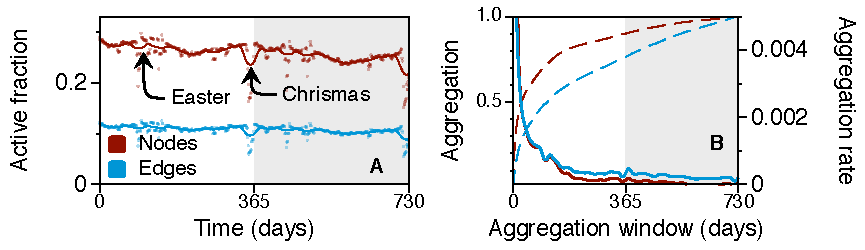
\includegraphics{Plos_S2AB.pdf}
\caption{\textbf{Panel A:} Daily activity of the network over two years.
Original data is shown as points and solid lines are local regressions of the original data.\\
\textbf{Panel B:} Time aggregation of the network for different aggregation windows.
Dashed lines show the fractions of nodes/edges in the aggregated network.
Solid lines are local regressions of the aggregation rates.
}
\label{fig:Plos_S1}
\end{center}
\end{figure}

Figure \ref{fig:Plos_S1} B gives a picture of the convergence of the network during the aggregation process, i.e. summing up the snapshots of the temporal system to obtain the static network representation.
The network is successively aggregated over more and more snapshots.
Dashed lines show the fractions of nodes and edges in the aggregated network, respectively.
The solid lines show the respective aggregation rates.
Since the latter are derivatives of the aggregation fractions, we do show a local regression of the aggregation rate to reduce noise in the signal.

The figure demonstrates that the aggregation rates for both nodes and edges becomes negligible after 1 year.
Therefore, we can assess a period of 1 year sufficient to provide stationarity of the system, i.e. the time span, after which only few more edges are added to the network.

\subsection{Simulated disease outbreaks}
Node rankings are of major importance for epidemiology.
We try to answer the question, if a constant ranking of node makes sense on a temporal network.
As a generic measure for the spreading potential of a node, we consider its range.
In analogy to section \ref{sec:network_analysis}, we define the range of a node in a temporal network as the size of its temporal out-component.
It is important to note that the out-component of each node depends on the time $t_0$, when it is measured.
In addition to that, the range of a node can depend on the particular spreading process, e.g. an epidemic, a chemical reaction or rumor spread.
More specifically, a spreading process can have a finite memory $d$ that shortens the ability of a node to maintain in a certain state over time.
In our context, this memory corresponds to the \emph{infectious period} $d$ of a disease, i.e. the time period, after the infection dies out if it is not carried over to another agent.
Computing the range combined with a finite infectious period mimics an SIR-type process, where the infectious period is related to the reciprocal recovery rate (see section \ref{sec:sir_model}).
For clarity reasons we do not solve differential equations for epidemics in this section and reduce the infection dynamics to assigning a discrete infection state -- susceptible, infected or recovered -- to each node in the network (see section \ref{sec:epi_networks}).
An infected node remains infected over the infectious period $d$.
Thus, the infection state of the whole network is given by the number of susceptible $S(t)$, infected $I(t)$ and recovered $R(t)$ nodes, respectively.

We define the \emph{temporal range} of a node $v$ by explicitly taking into account the time of (primary) infection and infectious period, i.e. $r(v,d,t_0)$.
Since there are no mixing states of nodes as in meta populations and we assume an infection probability $p=1$ for every contact edge, the range of a node is identical to the outbreak size $R(t=\infty )$. 

In summary, range and infectious period are intrinsically entangled on temporal networks
\begin{equation}\label{eq:range_and_inf_period}
\text{static network: } \; r(v) \;\;\; \rightarrow   \;\;\; \text{temporal network: } \; r(v,d) .
\end{equation}
For the rest of this work, we therefore use the notion \emph{range} and \emph{outbreak size} synonymously.
Although the temporal range should approach the static range for infinite memory, i.e. $r(v,d=\infty ) \rightarrow r(v)$, the static range of a node is in general not reached even in this case.
This is caused by causality of paths in temporal networks as explained in figure \ref{fig:temporal_network_principle}.

\subsubsection{Single outbreaks}
We discuss the outbreak pattern caused by single outbreaks in this section, while we discuss the properties of the set of all possible outbreak scenarios in the next section.
In order to analyze node ranges in the pig trade network, we use a modified breadth-first-search algorithm (see Appendix \ref{sec:implementation} for a brief summary of search algorithms for static networks).
Given a fixed infectious period, we mark a particular node $v$ to be infected at time $t_0$.
For every time step in the interval $[t_0,t_0+d]$, we identify the neighborhood $\mathcal{N}(v,t)$ and mark all susceptible nodes in $\mathcal{N}(v,t)$ as infected.
Infected nodes are marked as removed after the infectious period $k$ and do not contribute to further infections.
This procedure is repeated for all infected nodes as long as there are still infected nodes in the system.

\begin{SCfigure}
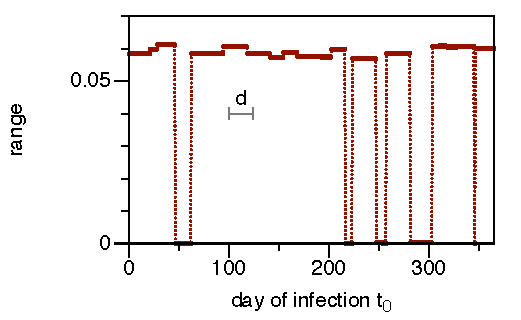
\includegraphics{exemplary_range.pdf}
\caption{Temporal variation in the range $r(v,d,t_0)$ of an exemplary node $v$ in the network over one year.
Although the range remains rather constant for most infection times, it vanishes for certain periods.
The grey interval corresponds to the fixed infectious period $d=24$~days.
}
\label{fig:range_exemplary}
\end{SCfigure}
%
Figure \ref{fig:range_exemplary} shows the range of an exemplary node in the network for different infection times $t_0$.
The infectious period is $d=24$ days.
For most infection times the example node can infect about $6~\%$ of the network.
The range distribution over time shows a similar bimodal pattern similar to the distribution over nodes for the static network in figure \ref{fig:node_range}.
This provides evidence that there is an infection path from the exemplary node to a connected component in the network.
It is important to stress that the concept of connected components does not translate to temporal networks in a straightforward manner (see section \ref{sec:conceptual_problems}).
Besides the bimodality itself, it remarkable that the majority of adjacent primary infection times cause outbreaks of similar size.

This feature is can be explained, if we underline the temporal sparsity of edges, i.e. nodes are likely to have only few contacts within one infectious period.
If the primarily infected node $v$ has no trade contact within the infectious period, the disease dies out.
Even if the disease is transferred to a successor node $w$ at a time $t_1$ within the interval $[t_0,t_0+d]$, the disease dies out, if there is not further trade contact within the period $[t_1+d]$ and so forth.
The regions of small/vanishing range in figure \ref{fig:range_exemplary} correspond to these scenarios.
On the other hand, if all successors of node $v$ have one or more trading contacts within their respective infectious periods, the disease can be transferred to a larger number of nodes.
The majority of small variations in $t_0$ implies stable ranges in the order of $d$ (the infectious period is shown by the grey line in figure \ref{fig:range_exemplary}).
If the degree of $v$ or a successor node in the infection chain is even larger than 1, even more secondary outbreaks are triggered and manifest themselves in smaller range fluctuations as for the long range values in \ref{fig:range_exemplary}.

We have seen in this section that a temporal degree of freedom adds a significant amount of complexity even to the outbreak pattern of a single node.
Now we focus on the set of all outbreak scenarios, i.e. the set of all initial conditions and variations in the infectious period as a parameter.
%
\subsubsection{Set of outbreak scenarios}
We apply the method discussed in the previous section to all nodes in the network.
As primary infection times, we consider all times within the first year in the dataset.
This ensures that even if a particular outbreak penetrates the second year, it will have died out within the observation period.
We restrict ourselves to infectious periods $d<56$~days, since this interval covers the infectious periods of the major livestock diseases \citep{Horst:1998wu,Konschake:2013js}.
Considering all nodes in the network as potential starting points for infections and all days in the first year of the dataset as possible starting times yields $10^9$ different initial conditions.
We denote the \emph{set of all outbreak scenarios} by $\mathcal{S}$.
More formally, let $\mathcal{G}=(V,\mathcal{E},T)$ be the temporal network of our dataset.
Then the set of all outbreaks is given by all possible initial conditions and parameters and the corresponding outbreak size, where the latter is identical to the range for our model:
\begin{equation}\label{eq:outbreak_set}
\mathcal{S}=\left\{ (v,t_0,d,r(v,d,t_0)): v \in V,t_0 \in T/2, d \leq 56  \right\}.
\end{equation}
%
In what follows, we will average over this set in different ways to immediately obtain information about the impact of infectious period, primary infection time or the starting node on disease spread.
Table \ref{tab:outbreak_set} shows a table representation of the set \eqref{eq:outbreak_set}.
%
\begin{table}[htb]
\sffamily
\begin{center}%\centering
\caption{Tabular data structure of the set of outbreak scenarios as defined by \eqref{eq:outbreak_set}.
We analyze 103,490 starting nodes for 365 times of primary infections and 56 different infectious periods yielding $10^9$ rows.
}
\begin{tabular*}{\hsize}{@{\extracolsep{\fill}}ccc|c}
\hline
~& initial conditions \& parameter  & ~ & result\\
\hline
Starting node & time of primary infection &infectious period & outbreak size \\
ID & $t_0$  &$d$ &$r(v,d,t_0)$  \\
\hline
1 & 1 & 1 & 58  \\
1 & 2 & 1 & 276  \\
\multicolumn{4}{c}{\vdots}\\%\vdots &\vdots &\vdots & \vdots \\
103,490 & 365 &56 & 72  \\
\hline
\end{tabular*}
\label{tab:outbreak_set}
\end{center}
\end{table}

Considering static networks, every node can cause an epidemic, if it is connected to other nodes in the network.
We have seen in the previous section that the time of primary infection has to be in an appropriate interval in temporal networks.
In addition, this constraint depends on the infectious period, since a disease with high infectious period is more likely to spread over the network than a disease with low infectious period.
We define the \emph{outbreak probability} $p_s(d)$ as the fraction of elements in $\mathcal{S}$ that causes a secondary outbreak at all, that is
\begin{equation}\label{eq:outbreak_prob}
p_s(k)=\frac{\abs{\left\{ x \subset \mathcal{S}: r(v,d,t_0) \in x >0, d=\mathrm{const.} \right\}}}{\abs{\mathcal{S}}} .
\end{equation}
Note that we compute the outbreak probability for each infectious period separately.

Figure \ref{fig:plosfig1} A shows the outbreak probability for different infectious periods.
For comparison, the outbreak probability in the static network is shown as dashed.
This is just the fraction of nodes with finite out degree and apparently the outbreak probability shows no dependence on the infectious period in the static case.
The outbreak probability saturates for sufficiently large infectious periods, but it is still only half as much as in the static case even for $d=56$.
%
\begin{figure}[htbp]
\begin{center}
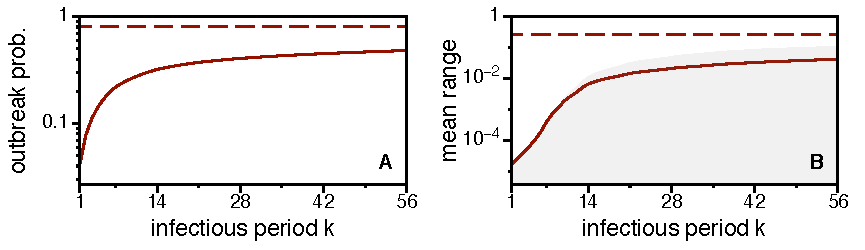
\includegraphics{Plos_fig1}
\caption{Outbreak probability (A) and mean range (B) for different infectious periods $d$ as solid lines.
Dashed lines correspond outbreak probability and mean outbreak size of the static network, respectively.
The grey shaded area in panel B shows the 50~\% confidence interval.}
\label{fig:plosfig1}
\end{center}
\end{figure}

In addition to the probability of an outbreak, we compute the expected size of the outbreaks.
The \emph{mean outbreak size} is an average over all starting nodes and all starting times in $\mathcal{S}$, i.e. $\mean{r(v,d,t_0)}_{v,t_0}$.
Figure \ref{fig:plosfig1} B shows the mean outbreak size and the 50~\% confidence interval (solid line and grey shaded area) and the mean outbreak size in the static network (dashed line).
As for the outbreak probability, we observe significant outbreak sizes only for $d>14$~days and the outbreak size is 6 times smaller than in the static case even for $d=56$~days.
In summary, the infectious period must be larger than 14~days to cause a severe outbreak and the static network approximation overestimates the size of outbreaks significantly.

\subsection{Node rankings}
This section is devoted to the analysis of the node ranking according to their respective ranges.
Rankings are very important for the implementation of vaccination and surveillance strategies, where the exact value of a certain measure for each node is not important.
%In fact, the \emph{ordering}
For every infectious period $d$, we average over all times of primary infection in \eqref{eq:outbreak_set}.
Thus, $b(v,d)=\mean{r(v,d,t_0)}_{t_0}$ is a function of the node and infectious period.
Ordering $b(v,d)$ for every $d$ in descending order gives a ranking $R(d)$ of the nodes according to their outbreak sizes, where $R(d)$ is an ordered set of nodes for every infectious period.
The question here is, whether these rankings remain stable, if the infectious period is changed.
%
\begin{SCfigure}
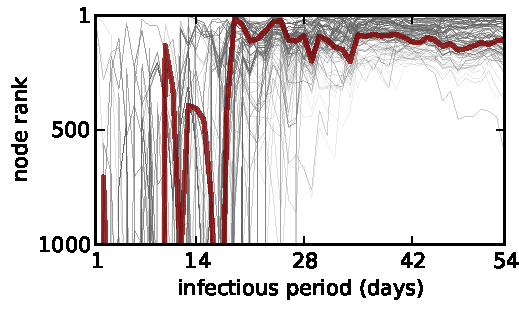
\includegraphics{vir_ranking.pdf}
\caption{Node ranking of the top 100 nodes over different infectious periods.
Rankings are computed by averaging \eqref{eq:outbreak_set} over the time of primary infection.
Top 100 nodes are the nodes with the largest outbreak sizes averaged over $d$ and $t_0$.
The rankings of an arbitrary node are shown in red for illustration purposes.}
\label{fig:ranking}
\end{SCfigure}

Figure \ref{fig:ranking} shows the ranking trajectories over different infectious periods of the top 100 nodes in the network. 
We define the top 100 nodes as the nodes with the largest outbreak size in $\mathcal{S}$ averaged over both $t_0$ and $d$, i.e. $\mean{r(v,d,t_0)}_{d,t_0}$.
An arbitrarily chosen node is shown in red for illustration purposes.
It should be noted that the rank of each node in the top 100 set can take any value in the figure, since the top 100 nodes are determined by averaging out the infectious period.

As the figure suggests, the ranking of nodes is unstable for small infectious periods ($d<21$~days).
This region is dominated by temporal fluctuations of the infection paths in the network.
Interestingly, the ranking approaches a stable region for $d>21$~days.
For $d>28$~days most nodes in the top 100 sample do not undergo significant rank changes any more.
This means that a ranking of nodes is reasonable for sufficiently large infectious periods.

\subsection{Inaccurate infectious periods and the robustness of node rankings}
Finding exact values of the infectious periods of a certain disease is often unachievable in real world scenarios.
Therefore, we look into the impact of variations in the infectious period on the ranking of nodes.
We consider pairs of rankings as defined in the previous section with different infectious periods, i.e. $R(d_1)$ and $R(d_2)$.

In order to compare two rankings, we could use measures of rank correlation, such as Spearman or Kendall rank correlation coefficients.
These turn out, however, to very sensitive to even small differences between two rankings.
Figure \ref{fig:ranking} suggests that even in the stable region where $d>28$~days node ranks remain similar, but not equal.
Computing Spearman or Kendall rank correlation coefficients for different infectious periods $(k_1,k_2)$ in our dataset would give vanishing values for almost all pairs $(d_1,d_2)$.
For that reason, we relax the requirements for similarity between to rankings.
Thus, we consider the \emph{intersection} between the sets of the respective upper samples of each ranking.
In other words, we examine whether the same nodes appear in the upper ranks of both the $R_{d_1}$ and the $R_{d_2}$ rankings.

We denote the subset of the upper $\tau $ ranks of $R(d)$ by $R_\tau (d)$.
As a similarity measure, we define the \emph{rank intersection} between two rankings $R_\tau (d_1)$ and $R_\tau (d_2)$ as
\begin{equation}\label{eq:rank_intersection}
s_\tau (d_1,d_2)=\frac{R_\tau (d_1) \cap R_\tau (d_2)}{\abs{R_\tau (d_1)}},
\end{equation}
that is the intersection between the sets of nodes normalized by the size of the top $n$ sample.
We get $s_\tau (d_1,d_2) =1$, if the upper $\tau $ nodes in the rankings $R(d_1)$ and $R(d_2)$ are identical.
On the other hand, $s_\tau (d_1,d_2) =0$ implies that ranks for $d_2$ and $d_2$ are completely different.

Using equation \eqref{eq:rank_intersection} yields a similarity matrix with $1540$ different combinations of infectious periods for our outbreak scenarios \eqref{eq:outbreak_set}.
Since particular combinations of infectious periods are nor relevant, we analyze the \emph{uncertainty} of the infectious period
\begin{equation}\label{eq:uncertainty_k}
\Delta d= \abs{d_1-d_2} .
\end{equation}
Now we average the entries of the similarity matrix over uncertainties and get the rank intersection
\begin{equation}\label{eq:robustness_k}
\tilde{s}_\tau (\Delta d)=\mean{s_\tau (d_1,d_2)}_{\abs{d_1-d_2}\leq \Delta d} .
\end{equation}
This rank intersection measures the robustness of a certain ranking against changes in the infectious period.
Therefore, we call this measure the \emph{rank robustness} a given uncertainty in the infectious period.
%
\begin{SCfigure}
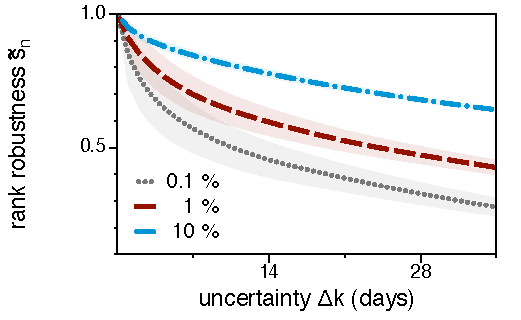
\includegraphics{Plos_fig4a.pdf}
\caption{Rank robustness vs. uncertainty in the infectious period for the upper $0.1$~\% (grey), $1$~\% (red) and $10$~\% (blue) of nodes in the network.
Shaded areas correspond to the $50$~\% confidence intervals.}
\label{fig:plos_fig4a}
\end{SCfigure}

For convenience, we express \eqref{eq:robustness_k} in terms of the upper \emph{fraction} of nodes instead of the upper nodes themselves.
That is, we replace the top $\tau $ nodes by the top fraction of nodes $n$:
\begin{equation}\label{eq:rank_robustness}
\tilde{s}_n (\Delta d)=\mean{s_n (d_1,d_2)}_{\abs{d_1-d_2}\leq \Delta d} .
\end{equation}
The same is implicitly done for rank intersection $s_n(d_1,d_2)$ \eqref{eq:robustness_k} and the node ranking $R_n(d)$.

We show the rank robustness for the fraction of the $0.1$~\%, $1$~\% and $10$~\% upper nodes in figure \ref{fig:plos_fig4a}.
These fractions correspond to approximately 100, 1000 and 10,000 nodes, respectively.
The $50$~\% confidence intervals of each curve are shown as shaded areas.
As expected, larger uncertainty in the infectious period generally leads to a decrease of rank robustness.
The decrease is small for the largest sample (blue), since the number of nodes in this sample is relatively large.
This guarantees that the same nodes are likely to be in all rankings $R_{10\%}(d)$ for all $d$.  
Consequently, the variation in rank robustness is relatively small (blue shaded area).
Considering the 0.1~\% sample (grey), it is remarkable that even for an uncertainty of 14~days, the robustness is still 50~\%.
As a smaller sample is more prone to fluctuations, variations of rank robustness are relatively large (grey shaded area).
The red curve shows an intermediate behavior.

\subsection{Temporal vs. static representation}
Since the analysis of a network using a data driven approach is computationally expensive, we compare the node rankings $R_n(k)$ to centrality measures for the static network representation as defined in section \ref{sec:micro_measures}.
We denote the upper $\tau $ nodes according to a static centrality measure as $C_\tau $.
Note that $C_\tau $ does not depend on the infectious period, since the latter plays no role in static networks.
In this work, we consider betweenness, closeness, degree centrality and range as centrality measures.
Following equation \eqref{eq:rank_intersection}, we define the \emph{centrality intersection} between the outbreak size ranking $R_\tau (d)$ and $C_\tau $ as
\begin{equation}\label{eq:centrality_intersection}
I_\tau (k)=\frac{R_\tau (d) \cap C_\tau}{\abs{C_\tau}},
\end{equation}
where $C_\tau $ is a substitute for the upper $\tau $ nodes of one particular centrality measure listed above.
%
\begin{figure}[htb]
\begin{center}
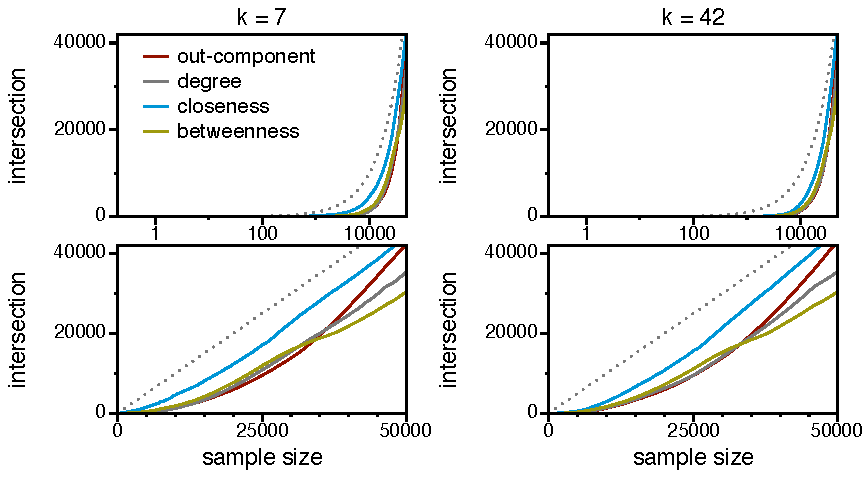
\includegraphics{Plos_fig5.pdf}
\caption{Intersection between outbreak size and different static centrality measures.
\textbf{Left~panel:}~infectious period $d=7$~days.
\textbf{Right~panel:}~infectious period $d=42$~days.
Top panels show $x$-log versions of the bottom panels. 
Dotted lines show data accordance $y=x$ for comparison.
The top panels demonstrate that finite intersections appear only for sample sizes of more than 1000 nodes.}
\label{fig:plos_fig5}
\end{center}
\end{figure}

In figure \ref{fig:plos_fig5}, we plot the centrality intersection \eqref{eq:centrality_intersection} for different static centrality measures and two exemplary infectious periods.
Upper panels are identical to the lower panels, but use logarithmic $x$-axes. 
The upper figures show that non vanishing intersections are taken for samples of at least 1000 nodes.
Consequently, the upper part of the ranked nodes does not coincide with high ranked nodes in any static centrality measure.
Intersection between outbreak size and static measures become significant for sample sizes of more than 10,000 nodes, i.e. about 10~\% of the network!
Although this fraction is rather large, the coincidence of centrality and outbreak size is still relatively small (lower panels, compare to dotted line).
The different centrality measures show similar intersections with the outbreak size.
An exception is closeness centrality, which performs significantly better than the other measures.
An explanation for this special role is that nodes with high closeness per definition are likely to infect other nodes within only few steps.
This way long static paths are avoided, i.e. the chance that one of these static paths is disrupted by causality is relatively low.
It should be noted that all features discussed above are almost identical for both infectious periods.

\paragraph{Summary of data aggregation methods\color{Cayenne}{.}}
We simulated an SIR-type disease on the livestock trade dataset and explicitly took into account the temporal dynamics of edges.
This yields a set of outbreak scenarios, which can be thought of as a scalar-field $r(v,d,t_0)$, where each triple $(v,d,t_0)$ is assigned an outbreak size $r$, if $r>0$.
A schematic sketch of this scalar-field is given in figure \ref{fig:Plos_parameter-space}.
%
\begin{SCfigure}
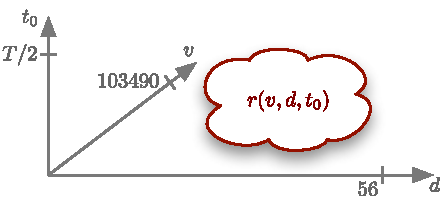
\includegraphics{Plos_parameter-space.pdf}
\caption{Scalar field representing the set of outbreak scenarios as defined in \eqref{eq:outbreak_set}.
Each combination of starting node $v$, starting time $t_0$ and infectious period $d$ yields an outbreak size $r(v,d,t_0)$.
The domain is bounded as defined in \eqref{eq:outbreak_set}.}
\label{fig:Plos_parameter-space}
\end{SCfigure}
%
Using the state space of figure \ref{fig:Plos_parameter-space}, we can summarize the different aggregation techniques used in this section as follows:
\begin{description}
\item [Exemplary outbreak:] Sum over all outbreak sizes for a cut through $r$ for constant $d$ and $v$ (see figure~\ref{fig:range_exemplary}).
\item [Outbreak probability:] State density of $r$ for every $d$-slice of the state space (see figure~\ref{fig:plosfig1}~A).
\item [Mean outbreak size:] The mean value of the field in every $d$-slice (see figure~\ref{fig:plosfig1}~B).
\item [Node ranking:] First, average over the $t_0$-axis. Afterwards ordering of nodes by largest outbreak size for every $d$-slice. See figure \ref{fig:ranking}.
\item [Infectious period uncertainty:] Comparison between pairs of node rankings. See figure~\ref{fig:plos_fig4a}.
\end{description}
%
The comparison to the static network representation (figure~\ref{fig:plos_fig5}) is obtained using intersections between pairs of node rankings in analogy to the estimation of uncertainty of the infectious period.

We conclude that although the temporal nature of the system results in strong fluctuations of the paths in the network, a ranking of nodes according to their range appears reasonable for sufficiently large infectious periods.
This ranking could not be reproduced using classical static centrality measures.
In addition to that, a static network view systematically overestimates disease outbreaks in the network.
Even for large infectious periods, we found the mean outbreak sizes to be six times smaller as for the static case.

\section{Graph centric temporal network analysis}\label{sec:PRL}
The previous section has shown that even the analysis of simple measures as node ranges is a complex endeavor.
While the previous section implicitly used a node centric approach to the system, we now introduce a \emph{graph centric} approach to temporal networks.
It is important to emphasize that the capability of static network analysis originates from the fact that the adjacency matrix provides a graph centric (``big picture'') of the system.
Therefore, a graph centric view on temporal networks contributes a key element for a theoretical framework for temporal systems.

As we have seen in section \ref{sec:paths_in_temporal_networks}, the static approximation of a temporal network falsely shows transitivity and therefore lacks a differentiation between causal and non causal paths.
We make use of adjacency matrix sequences (as defined by equation \eqref{eq:AdMatrixSequence}) and derive a method for the computation of causal paths.

This yields first the ranges of all nodes in the network (see sections \ref{sec:micro_measures} and \ref{sec:Plos}) and second information about the \emph{accessibility} between nodes.
In analogy to the static range defined in equation \eqref{eq:range_def}, the range of a node $v$ in a temporal network $\mathcal{G}=(V,\mathcal{E},T)$ can formally be defined as
\begin{equation}\label{eq:temporal_range_def}
r(v)=\frac{\left| \mathcal{H}(v) \right| }{N}, \; \text{ where } \; \mathcal{H}(v)=\{u \in V: v\rightsquigarrow u \},
\end{equation}
where $\mathcal{H}(v)$ is the horizon of node $v$ and $N$ the number of nodes in the network.

The set of all horizons in a network defines its \emph{accessibility graph}.
For static networks, the concept of accessibility was defined at the end of section \ref{sec:macro_measures}.
We extend the static accessibility approach to the explicit step by step derivation of accessibility in section \ref{sec:unfolding_static}.
This novel procedure is called \emph{unfolding} of accessibility.
Finally, we generalize the unfolding accessibility approach to temporal networks in section \ref{sec:unfolding_temporal}.

\subsection{Accessibility of static networks}\label{sec:unfolding_static}
We consider a static network $G=(V,E)$ with $N$ nodes and adjacency matrix $\mathbf{A}$.
The accessibility graph (or transitive closure) of $G$ is denoted by $G^*=(V,E^*)$, where $E^*$ contains an edge $(u,v)$, whenever $u\rightarrow v$.
The accessibility matrix -- i.e. the adjacency matrix of the accessibility graph -- can be computed using the cumulative matrix defined
\begin{equation*}%\label{eq:}
\mat{C}_n=\mat{A}+\mat{A}^2+\cdots + \mat{A}^n = \sum _{i=1} ^n \mat{A}^i .
\end{equation*}
This equation was already introduced in section \ref{sec:macro_measures}, equation \eqref{eq:cumulative_matrix}.
Every term $\mat{A}^i$ corresponds to a network where nodes are connected that have shortest path distance $i$ in G.
Figure \ref{fig:power_graphs} illustrates this observation.
%
\begin{SCfigure}
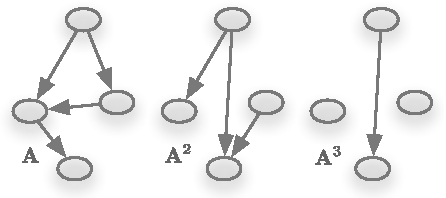
\includegraphics{Power-graphs.pdf}
\caption{Graph representations of different powers of an adjacency matrix.
The left panel shows the original graph $G$ with adjacency matrix $\mat{A}$.
Node pairs with distance 2 in $G$ are connected by an edge in the graph of $\mat{A}^2$ (middle).
The analogue for distance 3 is shown on the right panel.}
\label{fig:power_graphs}
\end{SCfigure}

In general, each power of an adjacency matrix contains the number of paths between node pairs as entries.
Since we are not interested in the actual \emph{number} of paths, we can treat the adjacency matrix as Boolean and use Boolean arithmetic and normal algebra.
Thus, the normalized cumulative matrix can be computed using
\begin{equation}\label{eq:static_boolean_acc}
\mathbf{P}_{n}=\bigvee _{i=1} ^{n} \mathbf{A}^i ,
\end{equation}
where the $i$-th power of the adjacency matrix is computed using the matrix product of two Boolean matrices $\mathbf{A}$ and $\mathbf{B}$ defined by 
\begin{align}\label{eq:boolean_product}
(\mat{A}\mat{B})_{ij}&=(a_{i1}\wedge b_{1j})\vee \dots \vee(a_{iN}\wedge b_{Nj}) \nonumber \\
&= \bigvee _{k=1}^N a_{ik} \wedge b_{kj} .
\end{align}
The adjacency matrix of the accessibility graph is given by $\mathbf{P}_{n=N-1}$.
We call $\mathbf{P}_{N-1}$ the \emph{accessibility matrix} of $G$.
Note that the index $N-1$ corresponds to the maximum path length in the network.
The graph $G^*$ given by $\mathbf{P}_{N-1}$ is the fully exploited accessibility graph.
We focus on accessibility for values other than $N-1$ below.

\paragraph{Properties of accessibility graphs\color{Cayenne}{.}}
In a \emph{connected} network $G$, the graph $G^*$ contains links between all node pairs, since all nodes are connected by a path.
Thus, $G^*$ is fully connected and the matrix $\mathbf{P}_{N-1}$ has only nonzero entries.
It follows from the transitivity of paths that all entries $(\mathbf{P})_{ii}$ are unity, since there is always a path from node $i$ to some other node $j$ and vice versa.
Consequently, $\mathbf{P}_{N-1}$ has $N^2$ nonzero entries in this case.
If the network $G$ is \emph{not connected}, the accessibility matrix can be transformed into a block diagonal form, where each block has only nonzero entries.
The total number of nonzero elements in this case is smaller than $N^2$.

%
\begin{figure}[htb]
\begin{center}
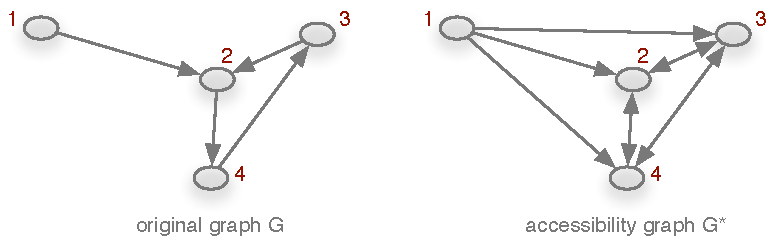
\includegraphics{Accessibility_principle_static.pdf}
\caption{A static network $G$ and its accessibility graph $G^*$.
The nodes 2, 3 and 4 are strongly connected in $G$ and form a clique in $G^*$.}
\label{fig:access_static}
\end{center}
\end{figure}
%
Figure \ref{fig:access_static} shows the accessibility graph of a static network.
The corresponding accessibility matrix is
\begin{equation*}
\mathbf{P}_N=\left(%
\begin{array}{c|ccc}%
0 & 1 & 1 & 1 \\
\hline 0 & 1 & 1 & 1 \\
0 & 1 & 1 & 1 \\
0 & 1 & 1 & 1
\end{array}\right) .
\end{equation*}
The nodes of the connected components in the adjacency matrix $\mathbf{A}$ form blocks in $\mathbf{P}_N$.

If the network $G$ is \emph{undirected}, every $\mathbf{P}_n$ has a non vanishing main diagonal for $n\geq 2$, if there are no isolated nodes.
This corresponds to the fact that there is always a path of length 2 from a node back to itself.
For the more general directed case, the main diagonal of $\mathbf{P}_{N-1}$ can contain 0 or 1 entries.

\paragraph{Shortest paths and unfolding accessibility\color{Cayenne}{.}}
Now we focus on the properties of the accessibility for the steps $\mathbf{P}_{n\leq N}$.
We explicitly take into account different values of $n$, i.e. we \emph{unfold} the accessibility graph.
The graph of $\mat{P}_1$ gives a graph containing paths of length 1, i.e. the adjacency matrix itself.
Analogues to figure \ref{fig:power_graphs}, the matrix $\mat{P}_2$ gives a graph containing paths of length 1 \emph{and} paths of length 2.
In principle, the procedure $\mat{P}_n \rightarrow \mat{P}_{n+1}$ corresponds to traversing the graph by paths of one more edge.
This is nothing other than a breadth-first-search (BFS) algorithm in the network (see appendix \ref{sec:implementation} for more details).
A similar method was used in early algorithms for computing shortest path lengths in networks \citep{Floyd:1962vo,Warshall:1962wr}.
At the moment, when the BFS-algorithm approaches the diameter $D$ of the network, the matrix $\mat{P}_n$ saturates and does not change for higher values of $n$.
Moreover, the accessibility matrix of a network is reached for $n=D$, so that
\begin{equation}\label{eq:diameter_sat}
\mat{P}_{D}\equiv \mat{P}_{D+1}\equiv \mat{P}_{N-1}.
\end{equation}
Hence, it is sufficient to compute only the first $D$ term in equation \eqref{eq:static_boolean_acc}.

The relation between the computation of accessibility and the BFS-algorithm suggests that this procedure contains information about the shortest path length distribution.
In order to reveal this correlation, we define the \emph{density} of a matrix $\mat{M}$ as the number of its nonzero elements, i.e.
\begin{equation}\label{eq:matrix_density}
\rho (\mat{M}) =\frac{\mathrm{nnz}(\mat{M})}{N^2}.
\end{equation}
In equation \eqref{eq:matrix_density} the number of nonzero elements is $\mathrm{nnz}(\mat{M})$ and $N$ is the dimension of $\mathbf{M}$.
As a special case, we define the \emph{path density} of a  network as the density of its accessibility matrix
\begin{equation}\label{eq:path_density}
\rho (\mat{P}_n) =\frac{\mathrm{nnz}(\mat{P}_n)}{N^2}.
\end{equation}
Note that the normalization in \eqref{eq:matrix_density} and \eqref{eq:path_density} are not $N(N-1)$, since we explicitly take into account self loops in the accessibility graph.
Ignoring these self loops could give values greater than 1 for connected graphs.

Now we address the relation between path density and shortest path distribution in a network.
In the case of the adjacency matrix, equation \eqref{eq:matrix_density} gives the edge density of the network.
It gives the probability that two randomly chosen nodes are connected by an edge.
It follows that the probability that these nodes are connected by a path of length $n$ is given by $\rho (\mat{A}^n)$.

Since the path density $\rho (\mat{P}_n)$ follows from a cumulative procedure, it corresponds to the probability that two randomly chosen nodes are connected by a length of length $l\leq n$.
Consequently, the path density is the cumulative distribution of shortest path lengths
\begin{equation}\label{eq:cumulative_distribution}
\rho (\mat{P}_n)=F(l\leq n)\equiv F_n .
\end{equation}
The shortest path length distribution follows from equation \eqref{eq:cumulative_distribution} by differentiation.
Since the step length is 1 by definition, the probability for a shortest path length $n$ is given by $f_n=(F_n-F_{n-1})$ and $F_0=0$.

It should be noted that the probabilities considered here can be normalized to 1 only for connected networks, because for connected networks $\rho (\mat{P}_{N-1})\equiv \mat{P}_D=1$.
In the case of unconnected networks, the saturation value is in general smaller than 1.
Therefore,  we treat the distribution \eqref{eq:cumulative_distribution} as an ``improper'' probability distribution, which is in general not normalized to unity.
In addition, we define the \emph{median} of $F_n$ as the value $n$ where $F_n=1/2 \; F_D$.

We make use of the relations discussed above in order to obtain information about the shortest path distribution.
The procedure is called \emph{Unfolding Accessibility}, because we explicitly analyze the step-by-step derivation of the accessibility matrix.
Although the concept of unfolding accessibility seems to make things unnecessarily complicated, it can be generalized to temporal networks.

But before we generalize the approach explained above to temporal networks, we illustrate the concept exemplarily for static \ER network.
We compute the shortest path length distribution of a directed \ER network of 1000 nodes and 2000 edges.
Figure \ref{fig:er_histo} shows the path density $\rho (\mat{P}_n)$ and the shortest path distribution.
The shortest path length distribution is identical to that of figure \ref{fig:ER_shortest_path_histogram} (section \ref{sec:er_model}).
%
\begin{figure}[htbp]
\begin{center}
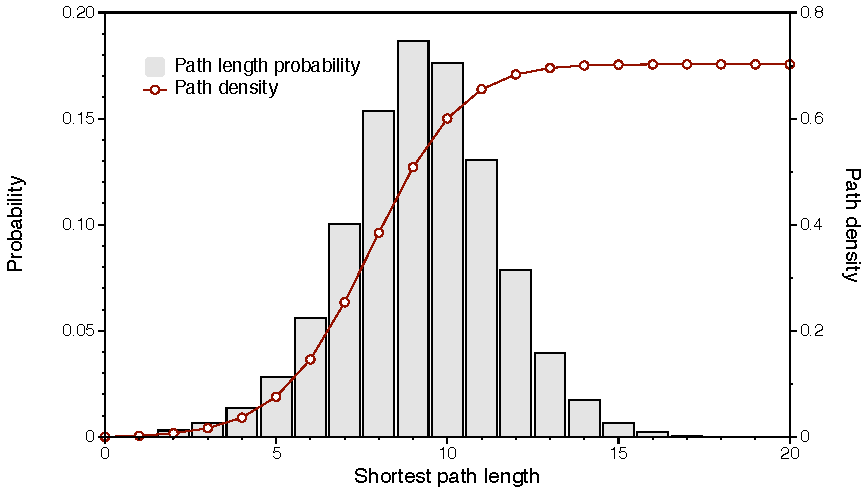
\includegraphics{ER_shortest_path_histo_double.pdf}
\caption{Path density (red line) and shortest path length distribution (grey histogram) for a directed \ER network with 1000 nodes and 2000 edges.
Mean value $8.18$, median $n=8$, diameter $D=18$, maximum path density $\rho (\mat{P}_D\approx 0.7)$.
The histogram is identical to that in figure \ref{sec:er_model}, where a different method was used.
}
\label{fig:er_histo}
\end{center}
\end{figure}
%





\subsection{Unfolding Accessibility of temporal networks}\label{sec:unfolding_temporal}


\subsection{Representative sample / characteristic time scale}

\subsection{Causal fidelity}

\subsection{Temporal and topological mixing patterns}

\subsection{Randomized models}\label{sec:randomized_models_tvg}





